% ============================================================================
% Parte 05 — Stewart, Precálculo 7.ª ed., §2.5 "Funciones lineales y modelos"
% (pp. 190–197 del libro; pp. 211–218 del PDF).
%
% Ejercicios elegidos (15) y página del libro:
%   Ej.  7 (p. 195) — Identificar funciones lineales
%   Ej.  9 (p. 195) — Identificar funciones lineales (no lineal)
%   Ej. 11 (p. 195) — Identificar funciones lineales (forma fraccionaria)
%   Ej. 15 (p. 195) — Trazar la gráfica de una función lineal
%   Ej. 17 (p. 195) — Trazar la gráfica de una función lineal (pendiente negativa)
%   Ej. 19 (p. 196) — Pendiente y razón de cambio
%   Ej. 25 (p. 196) — Pendiente y razón de cambio (coeficiente fraccionario)
%   Ej. 27 (p. 196) — Función lineal dada verbalmente
%   Ej. 29 (p. 196) — Función lineal dada verbalmente (pendiente e intersección)
%   Ej. 31 (p. 196) — Función lineal dada numéricamente (tabla)
%   Ej. 33 (p. 196) — Función lineal dada gráficamente (creciente)
%   Ej. 35 (p. 196) — Función lineal dada gráficamente (decreciente)
%   Ej. 39 (p. 196) — Aplicación: relleno sanitario
%   Ej. 41 (p. 196) — Aplicación: globo meteorológico
%   Ej. 43 (p. 196) — Aplicación: rampa para silla de ruedas
%
% Figuras extraídas del PDF: fig_p05_33.png, fig_p05_35.png (gráficas dadas en
% los ejercicios 33 y 35). Las demás gráficas se generan con pgfplots.
% ============================================================================
\documentclass[11pt]{article}
\usepackage[utf8]{inputenc}
\usepackage[spanish]{babel}
\usepackage[margin=2.3cm]{geometry}
\usepackage{amsmath,amssymb}
\usepackage{enumitem}
\usepackage{tcolorbox}
\tcbuselibrary{skins,breakable}
\usepackage{pgfplots}
\pgfplotsset{compat=1.18}
\usepackage{tikz}
\usepackage{graphicx}
\usepackage{array}
\usepackage[hidelinks]{hyperref}

% Notación española opcional (descomenta si quieres \sen en lugar de \sin)
% \DeclareMathOperator{\sen}{sen}
% \DeclareMathOperator{\tg}{tg}
% \DeclareMathOperator{\ctg}{ctg}

\newtcolorbox{sol}{colback=blue!5,colframe=blue!50!black,title=Solución paso a paso,breakable}
\newtcolorbox{teo}{colback=orange!8,colframe=orange!70!black,title=Teoría,breakable}
\newtcolorbox{nota}{colback=green!5,colframe=green!50!black,title=Idea clave,breakable}
\newtcolorbox{tip}{colback=yellow!10,colframe=yellow!60!black,title=Consejo,breakable}
\newtcolorbox{resp}{colback=red!5,colframe=red!50!black,title=Respuesta,breakable}
\newtcolorbox{reg}{colback=red!5,colframe=red!60!black,title=Regla,breakable}
\newtcolorbox{paso}[1]{colback=gray!5,colframe=gray!50!black,title={#1},breakable}

\graphicspath{{../images/}{images/}}
\newcommand{\sen}{\operatorname{sen}}

% babel spanish activa < y > y rompe TikZ/pgfplots (->, >=stealth)
\AtBeginDocument{\shorthandoff{<>}}

\begin{document}
\shorthandoff{<>}  % babel-spanish hace activos < y >; tikz/pgfplots los necesitan literales

\section*{Parte 05 — Funciones lineales y modelos (Stewart §2.5, pp. 190--197)}

\begin{teo}
\textbf{Método de la sección 2.5.}
\begin{enumerate}[leftmargin=*]
\item \textbf{Definición.} Una \textbf{función lineal} es una función de la forma $f(x)=ax+b$. Su gráfica es una recta de pendiente $a$ y punto de intersección $y$ igual a $b$.
\item \textbf{Identificar.} Desarrollá y simplificá la expresión. Es lineal solo si al final $x$ aparece únicamente a la primera potencia y con coeficiente constante; $x^2$, $\sqrt{x}$ o $x$ en el denominador la descalifican.
\item \textbf{Llevar a la forma $ax+b$.} Distribuí los productos y repartí el denominador numérico término a término; después leé $a$ (coeficiente de $x$) y $b$ (término independiente).
\item \textbf{Trazar la gráfica.} Como la gráfica es una recta, basta una tabla de valores, marcar dos de sus puntos y unirlos; los demás caen sobre la misma recta.
\item \textbf{Pendiente $=$ razón de cambio.} Para $f(x)=ax+b$, la pendiente de la gráfica y la razón de cambio de $f$ son ambas iguales a $a$. Si $a>0$ la cantidad aumenta; si $a<0$ disminuye.
\item \textbf{Construir un modelo.} Escribí $f(x)=ax+b$, tomá $a$ de la razón de cambio dada (o de dos puntos) y $b$ del valor inicial $f(0)$. Para preguntas del tipo ``¿cuándo llega a $V$?'' resolvé la ecuación $f(x)=V$.
\end{enumerate}
\end{teo}

\begin{tip}
Fórmulas que se repiten en toda la sección:
\begin{itemize}[leftmargin=*]
\item \textbf{Forma lineal:} $f(x)=ax+b$, con $a=$ pendiente $=$ razón de cambio y $b=f(0)=$ valor inicial.
\item \textbf{Pendiente por dos puntos:} $a=\dfrac{y_2-y_1}{x_2-x_1}=\dfrac{f(x_2)-f(x_1)}{x_2-x_1}$ (para una función lineal da lo mismo qué par de puntos se use).
\item \textbf{Repartir un denominador:} $\dfrac{px+q}{r}=\dfrac{p}{r}x+\dfrac{q}{r}$; \quad \textbf{distribuir:} $x(p+qx)=px+qx^2$.
\item \textbf{Unidades de la razón de cambio:} unidad de la salida entre unidad de la entrada (gal/min, pies/año, pulg/pulg, \dots).
\end{itemize}
\end{tip}

% ===========================================================================
\subsection*{Ejercicio 7 — Identificar funciones lineales}

\begin{quote}
\textbf{7--14 $\blacksquare$ Identificar funciones lineales}\quad Determine si la función dada es lineal. Si la función es lineal exprese la función en la forma $f(x)=ax+b$.

\textbf{7.} $f(x)=3+\tfrac{1}{3}x$
\end{quote}

\begin{paso}{Paso 1 --- Verificar la potencia de la variable}
\textbf{Qué hago:} reviso en qué potencia aparece $x$ en $3+\tfrac13 x$.

\textbf{¿De dónde sale?} Del enunciado: los dos términos son la constante $3$ y el término $\tfrac13 x$.

\textbf{¿Por qué?} Por la definición de función lineal, la expresión solo puede tener a $x$ elevada a la primera potencia.
\end{paso}

\begin{paso}{Paso 2 --- Reordenar a la forma $ax+b$}
\textbf{Qué hago:} conmuto los sumandos para dejar primero el término en $x$ y leo $a$ y $b$.

\textbf{¿De dónde sale?} De la expresión del paso 1; la suma es conmutativa, así que $3+\tfrac13x=\tfrac13x+3$.

\textbf{¿Por qué?} La forma $ax+b$ exhibe $a$ como coeficiente de $x$ y $b$ como término independiente.
\[
f(x)=\tfrac13 x+3,\qquad a=\tfrac13,\quad b=3.
\]
\end{paso}

\begin{resp}
Sí es lineal: $f(x)=\dfrac{1}{3}x+3$, con $a=\dfrac13$ y $b=3$.
\end{resp}

% ===========================================================================
\subsection*{Ejercicio 9 — Identificar funciones lineales (caso no lineal)}

\begin{quote}
\textbf{7--14 $\blacksquare$ Identificar funciones lineales}\quad Determine si la función dada es lineal. Si la función es lineal exprese la función en la forma $f(x)=ax+b$.

\textbf{9.} $f(x)=x(4-x)$
\end{quote}

\begin{paso}{Paso 1 --- Desarrollar el producto}
\textbf{Qué hago:} distribuyo $x$ sobre $4-x$.

\textbf{¿De dónde sale?} Del enunciado: $f(x)=x(4-x)$.

\textbf{¿Por qué?} Solo después de simplificar se puede comparar la expresión con la forma $ax+b$; un producto puede esconder potencias de $x$.
\[
f(x)=x\cdot 4-x\cdot x=4x-x^2
\]
\end{paso}

\begin{paso}{Paso 2 --- Comparar con la forma lineal}
\textbf{Qué hago:} constato que aparece el término $-x^2$.

\textbf{¿De dónde sale?} Del desarrollo del paso 1.

\textbf{¿Por qué?} La definición de función lineal exige que $x$ aparezca solo a la primera potencia, y $-x^2$ la incumple.
\end{paso}

\begin{resp}
No es lineal: al desarrollar queda $f(x)=4x-x^2$, con $x$ elevada al cuadrado.
\end{resp}

% ===========================================================================
\subsection*{Ejercicio 11 — Identificar funciones lineales (forma fraccionaria)}

\begin{quote}
\textbf{7--14 $\blacksquare$ Identificar funciones lineales}\quad Determine si la función dada es lineal. Si la función es lineal exprese la función en la forma $f(x)=ax+b$.

\textbf{11.} $f(x)=\dfrac{x+1}{5}$
\end{quote}

\begin{paso}{Paso 1 --- Repartir el denominador término a término}
\textbf{Qué hago:} aplico $\dfrac{p+q}{r}=\dfrac{p}{r}+\dfrac{q}{r}$ con denominador constante $5$.

\textbf{¿De dónde sale?} Del enunciado: numerador $x+1$, denominador $5$.

\textbf{¿Por qué?} Dividir entre la constante $5$ es multiplicar por $\tfrac15$, y la multiplicación se distribuye sobre la suma.
\[
f(x)=\frac{x}{5}+\frac{1}{5}=\frac15 x+\frac15
\]
\end{paso}

\begin{paso}{Paso 2 --- Leer $a$ y $b$}
\textbf{Qué hago:} identifico el coeficiente de $x$ y el término independiente.

\textbf{¿De dónde sale?} De la expresión del paso 1.

\textbf{¿Por qué?} La variable quedó a la primera potencia y el denominador es una constante (no contiene $x$), así que la función es lineal.
\end{paso}

\begin{resp}
Sí es lineal: $f(x)=\dfrac{1}{5}x+\dfrac{1}{5}$, con $a=\dfrac15$ y $b=\dfrac15$.
\end{resp}

% ===========================================================================
\subsection*{Ejercicio 15 — Trazar la gráfica de una función lineal}

\begin{quote}
\textbf{15--18 $\blacksquare$ Trazar la gráfica de funciones lineales}\quad Para la función lineal dada haga una tabla de valores y trace su gráfica. ¿Cuál es la pendiente de la gráfica?

\textbf{15.} $f(x)=2x-5$
\end{quote}

\begin{paso}{Paso 1 --- Tabla de valores}
\textbf{Qué hago:} evalúo $f(x)=2x-5$ en enteros consecutivos.

\textbf{¿De dónde sale?} De la fórmula del enunciado; por ejemplo $f(-2)=2(-2)-5=-4-5=-9$ y $f(3)=2(3)-5=6-5=1$.

\textbf{¿Por qué?} La tabla de valores es el procedimiento del ejemplo 2 de la sección para obtener puntos de la gráfica.
\begin{center}
\begin{tabular}{c|cccccc}
$x$ & $-2$ & $-1$ & $0$ & $1$ & $2$ & $3$\\ \hline
$f(x)$ & $-9$ & $-7$ & $-5$ & $-3$ & $-1$ & $1$
\end{tabular}
\end{center}
\end{paso}

\begin{paso}{Paso 2 --- Trazar la recta por dos puntos de la tabla}
\textbf{Qué hago:} marco $(0,-5)$ y $(3,1)$ y los uno con una recta.

\textbf{¿De dónde sale?} De dos filas de la tabla del paso 1.

\textbf{¿Por qué?} Como $f$ es lineal su gráfica es una recta, y dos puntos determinan una recta; los demás puntos de la tabla caen sobre ella.
\begin{center}
\begin{tikzpicture}
\begin{axis}[axis lines=middle, xlabel={$x$}, ylabel={$y$},
  xmin=-3, xmax=4, ymin=-10, ymax=3,
  width=8.5cm, height=6cm, grid=both, grid style={gray!20},
  xtick={-2,-1,1,2,3}, ytick={-9,-7,-5,-3,-1,1}, samples=2]
  \addplot[thick, red, domain=-2.5:3.5]{2*x-5};
  \addplot[only marks, mark=*, blue] coordinates {(0,-5) (3,1)};
\end{axis}
\end{tikzpicture}
\end{center}
\end{paso}

\begin{paso}{Paso 3 --- Leer la pendiente}
\textbf{Qué hago:} tomo el coeficiente de $x$ como pendiente.

\textbf{¿De dónde sale?} De $f(x)=2x-5$, comparada con $f(x)=ax+b$: $a=2$.

\textbf{¿Por qué?} Para una función lineal $f(x)=ax+b$ la pendiente de la gráfica es $a$ (recuadro ``Pendiente y razón de cambio''). Se comprueba con dos puntos: $\dfrac{1-(-5)}{3-0}=\dfrac{6}{3}=2$.
\end{paso}

\begin{resp}
La gráfica es la recta que pasa por $(0,-5)$ y $(3,1)$; su pendiente es $2$.
\end{resp}

% ===========================================================================
\subsection*{Ejercicio 17 — Trazar la gráfica (pendiente negativa)}

\begin{quote}
\textbf{15--18 $\blacksquare$ Trazar la gráfica de funciones lineales}\quad Para la función lineal dada haga una tabla de valores y trace su gráfica. ¿Cuál es la pendiente de la gráfica?

\textbf{17.} $r(t)=-\tfrac{2}{3}t+2$
\end{quote}

\begin{paso}{Paso 1 --- Tabla de valores con entradas múltiplos de 3}
\textbf{Qué hago:} evalúo $r(t)=-\tfrac23 t+2$ en $t=-3,0,3,6$.

\textbf{¿De dónde sale?} De la fórmula del enunciado: $r(-3)=-\tfrac23(-3)+2=2+2=4$ y $r(6)=-\tfrac23(6)+2=-4+2=-2$.

\textbf{¿Por qué?} Elegir múltiplos de $3$ hace que $-\tfrac23 t$ sea entero, y una tabla de valores es lo que pide el enunciado.
\begin{center}
\begin{tabular}{c|cccc}
$t$ & $-3$ & $0$ & $3$ & $6$\\ \hline
$r(t)$ & $4$ & $2$ & $0$ & $-2$
\end{tabular}
\end{center}
\end{paso}

\begin{paso}{Paso 2 --- Trazar la recta y leer la pendiente}
\textbf{Qué hago:} uno $(0,2)$ y $(3,0)$ con una recta y tomo el coeficiente de $t$ como pendiente.

\textbf{¿De dónde sale?} De la tabla del paso 1 y de la comparación $r(t)=-\tfrac23 t+2$ con $ax+b$: $a=-\tfrac23$.

\textbf{¿Por qué?} La gráfica de una función lineal es una recta de pendiente $a$; aquí $a<0$, así que la recta baja de izquierda a derecha.
\begin{center}
\begin{tikzpicture}
\begin{axis}[axis lines=middle, xlabel={$t$}, ylabel={$y$},
  xmin=-4, xmax=7, ymin=-3, ymax=5,
  width=8.5cm, height=5.5cm, grid=both, grid style={gray!20},
  xtick={-3,3,6}, ytick={-2,2,4}, samples=2]
  \addplot[thick, red, domain=-3.5:6.5]{-2/3*x+2};
  \addplot[only marks, mark=*, blue] coordinates {(0,2) (3,0)};
\end{axis}
\end{tikzpicture}
\end{center}
\end{paso}

\begin{resp}
La gráfica es la recta que pasa por $(0,2)$ y $(3,0)$; su pendiente es $-\dfrac{2}{3}$.
\end{resp}

% ===========================================================================
\subsection*{Ejercicio 19 — Pendiente y razón de cambio}

\begin{quote}
\textbf{19--26 $\blacksquare$ Pendiente y razón de cambio}\quad Se da una función lineal. \textbf{\textit{a}}) Trace la gráfica. \textbf{\textit{b}}) Encuentre la pendiente de la gráfica. \textbf{\textit{c}}) Determine la razón de cambio de la función.

\textbf{19.} $f(x)=2x-6$
\end{quote}

\begin{paso}{Paso 1 --- \textit{a}) Trazar la gráfica con dos puntos}
\textbf{Qué hago:} calculo la intersección con el eje $y$ y otro punto: $f(0)=-6$ y $f(3)=2(3)-6=0$.

\textbf{¿De dónde sale?} De sustituir $x=0$ y $x=3$ en $f(x)=2x-6$.

\textbf{¿Por qué?} La gráfica de una función lineal es una recta, y dos puntos la determinan.
\begin{center}
\begin{tikzpicture}
\begin{axis}[axis lines=middle, xlabel={$x$}, ylabel={$y$},
  xmin=-2, xmax=6, ymin=-8, ymax=4,
  width=8.5cm, height=5.5cm, grid=both, grid style={gray!20},
  xtick={-1,1,2,3,4,5}, ytick={-6,-4,-2,2}, samples=2]
  \addplot[thick, red, domain=-1.5:5.5]{2*x-6};
  \addplot[only marks, mark=*, blue] coordinates {(0,-6) (3,0)};
\end{axis}
\end{tikzpicture}
\end{center}
\end{paso}

\begin{paso}{Paso 2 --- \textit{b}) Pendiente y \textit{c}) razón de cambio}
\textbf{Qué hago:} leo $a$ en $f(x)=2x-6$ y lo uso como pendiente y como razón de cambio.

\textbf{¿De dónde sale?} De comparar $f(x)=2x-6$ con $f(x)=ax+b$: $a=2$, $b=-6$.

\textbf{¿Por qué?} Para $f(x)=ax+b$ se cumple $a=$ pendiente de la gráfica $=$ razón de cambio de $f$ (recuadro de la sección), porque la razón de cambio promedio entre dos puntos cualesquiera coincide con la pendiente.
\end{paso}

\begin{resp}
\textbf{\textit{a}}) Recta por $(0,-6)$ y $(3,0)$. \quad \textbf{\textit{b}}) Pendiente $=2$. \quad \textbf{\textit{c}}) Razón de cambio $=2$.
\end{resp}

% ===========================================================================
\subsection*{Ejercicio 25 — Pendiente y razón de cambio (coeficiente fraccionario)}

\begin{quote}
\textbf{19--26 $\blacksquare$ Pendiente y razón de cambio}\quad Se da una función lineal. \textbf{\textit{a}}) Trace la gráfica. \textbf{\textit{b}}) Encuentre la pendiente de la gráfica. \textbf{\textit{c}}) Determine la razón de cambio de la función.

\textbf{25.} $f(t)=-\tfrac{3}{2}t+2$
\end{quote}

\begin{paso}{Paso 1 --- \textit{a}) Dos puntos y la recta}
\textbf{Qué hago:} evalúo en $t=0$ y $t=2$: $f(0)=2$ y $f(2)=-\tfrac32(2)+2=-3+2=-1$.

\textbf{¿De dónde sale?} De sustituir en la fórmula del enunciado; elijo $t=2$ para que $-\tfrac32 t$ sea entero.

\textbf{¿Por qué?} Dos puntos determinan la recta que es la gráfica de una función lineal.
\begin{center}
\begin{tikzpicture}
\begin{axis}[axis lines=middle, xlabel={$t$}, ylabel={$y$},
  xmin=-3, xmax=5, ymin=-5, ymax=7,
  width=8.5cm, height=5.5cm, grid=both, grid style={gray!20},
  xtick={-2,-1,1,2,3,4}, ytick={-4,-2,2,4,6}, samples=2]
  \addplot[thick, red, domain=-2.5:4.5]{-1.5*x+2};
  \addplot[only marks, mark=*, blue] coordinates {(0,2) (2,-1)};
\end{axis}
\end{tikzpicture}
\end{center}
\end{paso}

\begin{paso}{Paso 2 --- \textit{b}) y \textit{c}) Leer $a$}
\textbf{Qué hago:} tomo el coeficiente de $t$.

\textbf{¿De dónde sale?} De $f(t)=-\tfrac32 t+2$ comparada con $ax+b$: $a=-\tfrac32$.

\textbf{¿Por qué?} En una función lineal la pendiente y la razón de cambio son ambas iguales a $a$; al ser $a<0$, $f$ decrece a razón de $\tfrac32$ unidades por unidad de $t$.
\end{paso}

\begin{resp}
\textbf{\textit{a}}) Recta por $(0,2)$ y $(2,-1)$. \quad \textbf{\textit{b}}) Pendiente $=-\dfrac32$. \quad \textbf{\textit{c}}) Razón de cambio $=-\dfrac32$.
\end{resp}

% ===========================================================================
\subsection*{Ejercicio 27 — Función lineal dada verbalmente}

\begin{quote}
\textbf{27--30 $\blacksquare$ Funciones lineales dadas verbalmente}\quad Se da una descripción verbal de una función lineal $f$. Exprese la función $f$ en la forma $f(x)=ax+b$.

\textbf{27.} La función lineal $f$ tiene razón de cambio 3 y valor inicial $-1$.
\end{quote}

\begin{paso}{Paso 1 --- Traducir ``razón de cambio'' al coeficiente $a$}
\textbf{Qué hago:} pongo $a=3$.

\textbf{¿De dónde sale?} Del enunciado: la razón de cambio es $3$.

\textbf{¿Por qué?} Para $f(x)=ax+b$, la razón de cambio de $f$ es exactamente $a$ (recuadro ``Pendiente y razón de cambio'').
\end{paso}

\begin{paso}{Paso 2 --- Traducir ``valor inicial'' al término $b$}
\textbf{Qué hago:} pongo $b=-1$ y armo la fórmula.

\textbf{¿De dónde sale?} Del enunciado: el valor inicial es $-1$, es decir $f(0)=-1$.

\textbf{¿Por qué?} $f(0)=a\cdot 0+b=b$, así que el valor inicial es el término independiente.
\[
f(x)=3x-1
\]
\end{paso}

\begin{resp}
$f(x)=3x-1$
\end{resp}

% ===========================================================================
\subsection*{Ejercicio 29 — Función lineal dada verbalmente (pendiente e intersección)}

\begin{quote}
\textbf{27--30 $\blacksquare$ Funciones lineales dadas verbalmente}\quad Se da una descripción verbal de una función lineal $f$. Exprese la función $f$ en la forma $f(x)=ax+b$.

\textbf{29.} La gráfica de la función lineal $h$ tiene pendiente $\tfrac12$ y punto de intersección 3.
\end{quote}

\begin{paso}{Paso 1 --- La pendiente es el coeficiente de $x$}
\textbf{Qué hago:} pongo $a=\tfrac12$.

\textbf{¿De dónde sale?} Del enunciado: la pendiente de la gráfica es $\tfrac12$.

\textbf{¿Por qué?} La gráfica de $h(x)=ax+b$ es una recta de pendiente $a$.
\end{paso}

\begin{paso}{Paso 2 --- El punto de intersección $y$ es $b$}
\textbf{Qué hago:} pongo $b=3$ y escribo la función.

\textbf{¿De dónde sale?} Del enunciado: el punto de intersección (con el eje $y$) es $3$.

\textbf{¿Por qué?} En $h(x)=ax+b$ la recta corta el eje $y$ en $b$, porque $h(0)=b$.
\[
h(x)=\tfrac12 x+3
\]
\end{paso}

\begin{resp}
$h(x)=\dfrac{1}{2}x+3$
\end{resp}

% ===========================================================================
\subsection*{Ejercicio 31 — Función lineal dada numéricamente}

\begin{quote}
\textbf{31--32 $\blacksquare$ Funciones lineales dadas numéricamente}\quad Se da una tabla de valores para una función lineal $f$. \textbf{\textit{a}}) Encuentre la razón de cambio de $f$. \textbf{\textit{b}}) Exprese $f$ en la forma $f(x)=ax+b$.

\textbf{31.}
\begin{center}
\begin{tabular}{c|c}
$x$ & $f(x)$\\ \hline
$0$ & $7$\\
$2$ & $10$\\
$4$ & $13$\\
$6$ & $16$\\
$8$ & $19$
\end{tabular}
\end{center}
\end{quote}

\begin{paso}{Paso 1 --- \textit{a}) Razón de cambio con dos filas de la tabla}
\textbf{Qué hago:} aplico $a=\dfrac{f(x_2)-f(x_1)}{x_2-x_1}$ a las filas $x=0$ y $x=2$.

\textbf{¿De dónde sale?} De la tabla: $f(0)=7$ y $f(2)=10$.

\textbf{¿Por qué?} En una función lineal la razón de cambio promedio es igual entre dos puntos cualesquiera, así que basta un par.
\[
a=\frac{10-7}{2-0}=\frac{3}{2}
\]
\end{paso}

\begin{paso}{Paso 2 --- Confirmar que la razón es constante}
\textbf{Qué hago:} repito el cálculo con el último par: $x=6$ y $x=8$.

\textbf{¿De dónde sale?} De la tabla: $f(6)=16$ y $f(8)=19$.

\textbf{¿Por qué?} Es la verificación de que los datos sí corresponden a una función lineal (razón de cambio constante).
\[
\frac{19-16}{8-6}=\frac{3}{2}
\]
\end{paso}

\begin{paso}{Paso 3 --- \textit{b}) Armar $f(x)=ax+b$}
\textbf{Qué hago:} uso $a=\tfrac32$ del paso 1 y tomo $b=f(0)$ directamente de la tabla.

\textbf{¿De dónde sale?} La primera fila de la tabla da $f(0)=7$, y $f(0)=b$.

\textbf{¿Por qué?} El término independiente de una función lineal es su valor en $x=0$. Comprobación: $f(8)=\tfrac32(8)+7=12+7=19$, que coincide con la tabla.
\[
f(x)=\tfrac32 x+7
\]
\end{paso}

\begin{resp}
\textbf{\textit{a}}) Razón de cambio $=\dfrac32$. \quad \textbf{\textit{b}}) $f(x)=\dfrac{3}{2}x+7$.
\end{resp}

% ===========================================================================
\subsection*{Ejercicio 33 — Función lineal dada gráficamente (creciente)}

\begin{quote}
\textbf{33--36 $\blacksquare$ Funciones lineales dadas gráficamente}\quad Se da la gráfica de una función lineal $f$. \textbf{\textit{a}}) Encuentre la razón de cambio de $f$. \textbf{\textit{b}}) Exprese $f$ en la forma $f(x)=ax+b$.

\textbf{33.}
\begin{center}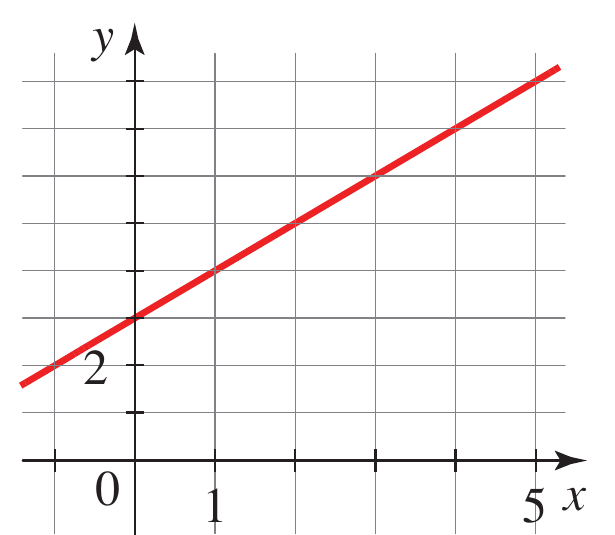
\includegraphics[width=0.5\textwidth]{fig_p05_33.png}\end{center}
\end{quote}

\begin{paso}{Paso 1 --- Leer dos puntos de la recta}
\textbf{Qué hago:} localizo dos puntos con coordenadas enteras sobre la recta.

\textbf{¿De dónde sale?} De la gráfica: en el eje $y$ están marcadas las unidades (la marca $2$ está a dos divisiones del origen), y en el eje $x$ las marcas $1$ y $5$. La recta pasa por $(0,3)$ y por $(5,8)$.

\textbf{¿Por qué?} Para determinar una recta alcanza con dos de sus puntos, y conviene tomarlos sobre cruces de la cuadrícula para leerlos sin error.
\end{paso}

\begin{paso}{Paso 2 --- \textit{a}) Calcular la razón de cambio}
\textbf{Qué hago:} aplico $a=\dfrac{y_2-y_1}{x_2-x_1}$ a los puntos del paso 1.

\textbf{¿De dónde sale?} De $(x_1,y_1)=(0,3)$ y $(x_2,y_2)=(5,8)$.

\textbf{¿Por qué?} En una función lineal la pendiente de la gráfica es la razón de cambio de la función.
\[
a=\frac{8-3}{5-0}=\frac{5}{5}=1
\]
\end{paso}

\begin{paso}{Paso 3 --- \textit{b}) Escribir $f$}
\textbf{Qué hago:} tomo $b$ como la ordenada del corte con el eje $y$.

\textbf{¿De dónde sale?} Del paso 1: la recta corta el eje $y$ en $3$, o sea $f(0)=3$.

\textbf{¿Por qué?} En $f(x)=ax+b$ el punto de intersección $y$ es $b$.
\[
f(x)=x+3
\]
\end{paso}

\begin{resp}
\textbf{\textit{a}}) Razón de cambio $=1$. \quad \textbf{\textit{b}}) $f(x)=x+3$.
\end{resp}

% ===========================================================================
\subsection*{Ejercicio 35 — Función lineal dada gráficamente (decreciente)}

\begin{quote}
\textbf{33--36 $\blacksquare$ Funciones lineales dadas gráficamente}\quad Se da la gráfica de una función lineal $f$. \textbf{\textit{a}}) Encuentre la razón de cambio de $f$. \textbf{\textit{b}}) Exprese $f$ en la forma $f(x)=ax+b$.

\textbf{35.}
\begin{center}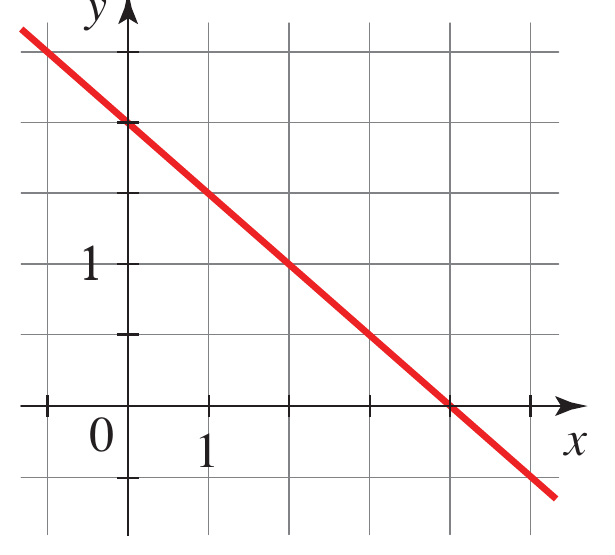
\includegraphics[width=0.5\textwidth]{fig_p05_35.png}\end{center}
\end{quote}

\begin{paso}{Paso 1 --- Leer la escala y dos puntos}
\textbf{Qué hago:} identifico la escala de cada eje y luego dos puntos de la recta.

\textbf{¿De dónde sale?} De la gráfica: la marca $1$ del eje $y$ está dos divisiones arriba del origen (cada división vale $\tfrac12$), y la marca $1$ del eje $x$ está una división a la derecha. La recta corta el eje $y$ en $2$ y corta el eje $x$ en $4$.

\textbf{¿Por qué?} Antes de calcular pendientes hay que fijar cuánto vale cada división; las divisiones de los dos ejes no representan aquí la misma cantidad.
\end{paso}

\begin{paso}{Paso 2 --- \textit{a}) Calcular la razón de cambio}
\textbf{Qué hago:} aplico la fórmula de la pendiente a $(0,2)$ y $(4,0)$.

\textbf{¿De dónde sale?} De los dos cortes con los ejes leídos en el paso 1.

\textbf{¿Por qué?} La pendiente de la gráfica de una función lineal es su razón de cambio; el signo negativo refleja que la recta baja.
\[
a=\frac{0-2}{4-0}=-\frac{2}{4}=-\frac12
\]
\end{paso}

\begin{paso}{Paso 3 --- \textit{b}) Escribir $f$}
\textbf{Qué hago:} uso $a=-\tfrac12$ y $b=2$.

\textbf{¿De dónde sale?} Del paso 2 y del corte con el eje $y$ en $2$, es decir $f(0)=2$.

\textbf{¿Por qué?} $f(0)=b$. Comprobación: $f(4)=-\tfrac12(4)+2=-2+2=0$, que es el corte con el eje $x$ leído en la gráfica.
\[
f(x)=-\tfrac12 x+2
\]
\end{paso}

\begin{resp}
\textbf{\textit{a}}) Razón de cambio $=-\dfrac12$. \quad \textbf{\textit{b}}) $f(x)=-\dfrac{1}{2}x+2$.
\end{resp}

% ===========================================================================
\subsection*{Ejercicio 39 — Aplicación: relleno sanitario}

\begin{quote}
\textbf{39. Relleno sanitario}\quad La cantidad de basura en un relleno sanitario del condado se modela por la función
\[
T(x)=150x+32\,000
\]
donde $x$ es el número de años desde 1996 y $T(x)$ se mide en millas de toneladas.

\textbf{\textit{a}}) Trace una gráfica de $T$.

\textbf{\textit{b}}) ¿Cuál es la pendiente de la gráfica?

\textbf{\textit{c}}) ¿A qué razón aumenta por año la cantidad de basura en el relleno sanitario?
\end{quote}

\begin{nota}
En esta edición en español la unidad aparece impresa como ``millas de toneladas''. Es una errata por \emph{miles de toneladas}: la unidad no afecta los cálculos, solo cómo se enuncia la respuesta del inciso \textit{c}).
\end{nota}

\begin{paso}{Paso 1 --- \textit{a}) Dos puntos y la gráfica}
\textbf{Qué hago:} evalúo $T(0)=32\,000$ y $T(20)=150(20)+32\,000=3000+32\,000=35\,000$.

\textbf{¿De dónde sale?} De sustituir $x=0$ (año 1996) y $x=20$ (año 2016) en $T(x)=150x+32\,000$.

\textbf{¿Por qué?} $T$ es lineal, así que su gráfica es la recta que pasa por esos dos puntos.
\begin{center}
\begin{tikzpicture}
\begin{axis}[axis lines=left, xlabel={$x$ (años desde 1996)}, ylabel={$T(x)$ (miles de toneladas)},
  xmin=0, xmax=22, ymin=31000, ymax=35500,
  width=9.5cm, height=5.5cm, grid=both, grid style={gray!20},
  xtick={0,5,10,15,20}, ytick={32000,33000,34000,35000},
  scaled y ticks=false, y tick label style={/pgf/number format/1000 sep={\,}}, samples=2]
  \addplot[thick, red, domain=0:21]{150*x+32000};
  \addplot[only marks, mark=*, blue] coordinates {(0,32000) (20,35000)};
\end{axis}
\end{tikzpicture}
\end{center}
\end{paso}

\begin{paso}{Paso 2 --- \textit{b}) Pendiente y \textit{c}) razón de cambio}
\textbf{Qué hago:} leo el coeficiente de $x$ y le pongo unidades.

\textbf{¿De dónde sale?} De comparar $T(x)=150x+32\,000$ con $ax+b$: $a=150$, $b=32\,000$.

\textbf{¿Por qué?} Para una función lineal, $a$ es a la vez la pendiente de la gráfica y la razón de cambio; como $x$ está en años y $T$ en miles de toneladas, las unidades son miles de toneladas por año, y $a>0$ indica aumento.
\end{paso}

\begin{resp}
\textbf{\textit{a}}) Recta por $(0,32\,000)$ y $(20,35\,000)$. \quad \textbf{\textit{b}}) Pendiente $=150$. \quad \textbf{\textit{c}}) La basura aumenta a razón de $150$ miles de toneladas por año.
\end{resp}

% ===========================================================================
\subsection*{Ejercicio 41 — Aplicación: globo meteorológico}

\begin{quote}
\textbf{41. Globo meteorológico}\quad Los globos meteorológicos se llenan de hidrógeno y se liberan en diferentes sitios para medir y transmitir datos de condiciones tales como la temperatura y la presión del aire. Un globo meteorológico se llena con hidrógeno a una velocidad de $0.5$ pies$^3$/s. Inicialmente el globo contiene 2 pies$^3$ de hidrógeno.

\textbf{\textit{a}}) Encuentre una función lineal $V$ que modele el volumen de hidrógeno en el globo en cualquier tiempo $t$.

\textbf{\textit{b}}) Si el globo tiene una capacidad de 15 pies$^3$, ¿cuánto tiempo tarda en llenarse completamente?
\end{quote}

\begin{paso}{Paso 1 --- \textit{a}) Plantear el modelo y fijar $a$}
\textbf{Qué hago:} escribo $V(t)=at+b$ y tomo $a=0.5$.

\textbf{¿De dónde sale?} Del enunciado: el hidrógeno entra a $0.5$ pies$^3$ por segundo, que es la razón de cambio del volumen.

\textbf{¿Por qué?} La razón de llenado es constante, y en un modelo lineal la razón de cambio es el coeficiente $a$ (ejemplo 4 de la sección).
\end{paso}

\begin{paso}{Paso 2 --- Fijar $b$ con la condición inicial}
\textbf{Qué hago:} impongo $V(0)=2$.

\textbf{¿De dónde sale?} Del enunciado: inicialmente ($t=0$) el globo contiene 2 pies$^3$.

\textbf{¿Por qué?} $V(0)=a\cdot 0+b=b$, así que el valor inicial es directamente $b$.
\[
V(t)=0.5t+2
\]
\end{paso}

\begin{paso}{Paso 3 --- \textit{b}) Resolver $V(t)=15$}
\textbf{Qué hago:} planteo la ecuación con la capacidad y despejo $t$.

\textbf{¿De dónde sale?} De la capacidad dada, 15 pies$^3$, y del modelo del paso 2.

\textbf{¿Por qué?} El globo está lleno cuando el volumen alcanza la capacidad. Comprobación: $0.5(26)+2=13+2=15$.
\[
15=0.5t+2 \;\Longrightarrow\; 13=0.5t \;\Longrightarrow\; t=26
\]
\end{paso}

\begin{resp}
\textbf{\textit{a}}) $V(t)=0.5t+2$ (volumen en pies$^3$, $t$ en segundos). \quad \textbf{\textit{b}}) Tarda $26$ segundos en llenarse.
\end{resp}

% ===========================================================================
\subsection*{Ejercicio 43 — Aplicación: rampa para silla de ruedas}

\begin{quote}
\textbf{43. Rampa para silla de ruedas}\quad Un comedor local debe construir una rampa para sillas de ruedas para facilitar el acceso de discapacitados al restaurante. Los códigos de construcción federales requieren que una rampa para silla de ruedas tenga una elevación máxima de 1 pulg por cada 12 pulg de distancia horizontal.

\textbf{\textit{a}}) ¿Cuál es la pendiente máxima permitida para una rampa para silla de ruedas? Suponiendo que la rampa tiene la elevación máxima encuentre una función lineal $H$ que modele la altura de la rampa sobre el suelo en función de la distancia horizontal $x$.

\textbf{\textit{b}}) Si el espacio disponible para construir una rampa es de 150 pulg de ancho, ¿qué elevación alcanza la rampa?
\end{quote}

\begin{paso}{Paso 1 --- \textit{a}) Traducir el código a una pendiente}
\textbf{Qué hago:} formo la razón elevación/desplazamiento.

\textbf{¿De dónde sale?} Del enunciado: 1 pulg de elevación por cada 12 pulg horizontales.

\textbf{¿Por qué?} La pendiente es el cambio vertical entre el cambio horizontal; es el mismo cálculo ``subida entre desplazamiento'' del ejemplo 5 (escalera).
\[
a=\frac{1\ \text{pulg}}{12\ \text{pulg}}=\frac{1}{12}
\]
\end{paso}

\begin{paso}{Paso 2 --- Fijar $b$ con el punto de partida de la rampa}
\textbf{Qué hago:} escribo $H(x)=ax+b$ e impongo $H(0)=0$.

\textbf{¿De dónde sale?} La rampa arranca al nivel del suelo: a distancia horizontal $0$ su altura es $0$.

\textbf{¿Por qué?} $H(0)=b$, así que $b=0$ y el modelo queda con un solo término.
\[
H(x)=\tfrac{1}{12}x
\]
\end{paso}

\begin{paso}{Paso 3 --- \textit{b}) Evaluar en $x=150$}
\textbf{Qué hago:} sustituyo la distancia horizontal disponible en el modelo.

\textbf{¿De dónde sale?} Del enunciado: el espacio es de 150 pulg de ancho.

\textbf{¿Por qué?} La altura alcanzada al final de la rampa es el valor del modelo en el extremo horizontal.
\[
H(150)=\frac{150}{12}=12.5
\]
\end{paso}

\begin{resp}
\textbf{\textit{a}}) Pendiente máxima $=\dfrac{1}{12}$, y el modelo es $H(x)=\dfrac{1}{12}x$ (con $x$ y $H(x)$ en pulgadas). \quad \textbf{\textit{b}}) La rampa alcanza $12.5$ pulg de elevación.
\end{resp}

\end{document}
